%%%%%%%%%%%%%%%%%%%%%%%%%%%%%%%%%%%%%%%%%%%%%%%%%%%%%%%%%%%%%%%%%%%%%%
% Problem statement
\begin{statement}[
  problempoints=70,
  timelimit=1 second,
  memorylimit=512 MiB,
]{Grudanje}

\setlength\intextsep{-0.1cm}
\begin{wrapfigure}[7]{r}{0.25\textwidth}
\centering
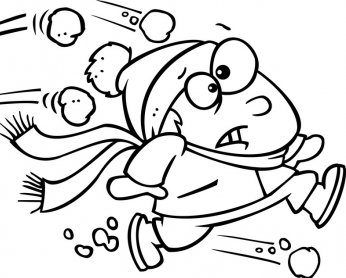
\includegraphics[width=0.25\textwidth]{img/gruda.png}
\end{wrapfigure}

%\subsection

Patrik loves to study the words in English language. He especially loves words
that contain exactly $N$ letters. When he sees such a word, he instantly starts
observing $Q$ of its subwords and for each of those subwords he determines
whether all of its letters are distinct. If that is the case for each of the
$Q$ subwords, then he considers the original word to be perfect.

  Krešimir doesn't love studying English words, he loves to throw snowballs at
Patrik instead. On a cold, winter morning, he was walking around town
carrying exactly $N$ snowballs and stumbled upon Patrik who was observing a
giant $N$-lettered word that was written on the wall by some hooligans.  What
a coincidence\dots

Krešimir fiercely threw the first snowball in Patrik's direction, but Patrick
skillfully dodged the snowball so it hit and completely
covered the $p_1$-st letter of the word on a wall. In a similar manner,
Krešimir failed to hit Patrik with the next $(N-1)$ snowballs. More precisely,
his $i$-th snowball missed Patrik and completely covered the $p_i$-th letter
of the word on a wall. Interestingly enough, after Krešimir threw all of the
snowballs, the entire word was covered in snow.

Patrik glanced at the completely covered word and concluded that it was perfect.
Therefore, he needed to slightly alter his definition of a perfect word. The
word is perfect in none of the $Q$ subwords contain two equal letters that are
not covered in snow. Now he wants to know after which snowball (possibly
zero) did the word on the wall become perfect.

%%%%%%%%%%%%%%%%%%%%%%%%%%%%%%%%%%%%%%%%%%%%%%%%%%%%%%%%%%%%%%%%%%%%%%
% Input
\subsection*{Input}
The first line contains a word that consists of $N$ $(1 \le N \le 10^5)$
lowercase letters from the English alphabet.

The second line contains an integer $Q$ $(1 \le Q \le 10^5)$ from the task
description.

The $i$-th of the next $Q$ lines contains two integers $a_i$ and $b_i$
$(1 \le a_i \le b_i \le N)$ which denote that the $i$-th of the $Q$ subwords
from the task description spans from $a_i$-th to the $b_i$-th letter of the
word on a wall.

The next line contains $N$ different integers $p_i$ $(1 \le p_i \le N)$ from
the task description.

%%%%%%%%%%%%%%%%%%%%%%%%%%%%%%%%%%%%%%%%%%%%%%%%%%%%%%%%%%%%%%%%%%%%%%
% Output
\subsection*{Output}
In the only line you should output after which snowball (possibly zero) did
the word on the wall become perfect.

%%%%%%%%%%%%%%%%%%%%%%%%%%%%%%%%%%%%%%%%%%%%%%%%%%%%%%%%%%%%%%%%%%%%%%
% Scoring
\subsection*{Scoring}
In test cases worth a total of 14 points, it will hold $1 \le N, Q \le 500$. \\
In test cases worth additional 21 points, it will hold $1 \le N, Q \le 3000$. \\
In test cases worth additional 14 points the word will only contain letters
\texttt{'a'}.

%%%%%%%%%%%%%%%%%%%%%%%%%%%%%%%%%%%%%%%%%%%%%%%%%%%%%%%%%%%%%%%%%%%%%%
% Examples
\subsection*{Examples}
\begin{tabularx}{\textwidth}{X'X'X}
\sampleinputs{test/grudanje.dummy.in.1}{test/grudanje.dummy.out.1} &
\sampleinputs{test/grudanje.dummy.in.2}{test/grudanje.dummy.out.2} &
\sampleinputs{test/grudanje.dummy.in.3}{test/grudanje.dummy.out.3}
\end{tabularx}

\textbf{Clarification of the second example:}

The state of the word on the wall after each thrown snowball is:\\
 \texttt{abbab*ab} \\
 \texttt{ab*ab*ab} \\
 \texttt{ab*a**ab} \\
 \texttt{*b*a**ab} \\
 \texttt{*b****ab} \\
 \texttt{******ab} \\
 \texttt{*******b} \\
 \texttt{********}

%%%%%%%%%%%%%%%%%%%%%%%%%%%%%%%%%%%%%%%%%%%%%%%%%%%%%%%%%%%%%%%%%%%%%%
% We're done
\end{statement}

%%% Local Variables:
%%% mode: latex
%%% mode: flyspell
%%% ispell-local-dictionary: "croatian"
%%% TeX-master: "../hio.tex"
%%% End:
